\documentclass[../ai_in_finance]{subfiles}
\usepackage[margin=1in]{geometry}
\usepackage{tikz}
\usetikzlibrary{positioning}
\usepackage{amsmath}
\usepackage{amssymb}
\usepackage{booktabs}
\usepackage{floatrow}
\usepackage{draftwatermark}

\SetWatermarkText{Wulin.Suo@Queensu.ca}
\SetWatermarkScale{1.4}
\SetWatermarkColor{gray!35}
\SetWatermarkAngle{90}
\SetWatermarkHorCenter{0.94\paperwidth}
\SetWatermarkVerCenter{0.5\paperheight}

\usepackage{makeidx}
\makeindex

\begin{document}

\chapter{Portfolio Theory and Asset Allocation}

\section{Introduction}

Chapter 2 introduced a two-asset portfolio to teach the mechanics of Python, and found, almost as an aside, that combining two negatively correlated assets produced a portfolio considerably less volatile than either asset held alone. This chapter returns to that observation and treats it as the central question of a whole field: given a set of available assets, their expected returns, and how they move together, what is the best way to combine them?

Portfolio theory answers this question with a specific, quantitative definition of ``best'': the highest expected return for a given level of risk. This chapter develops the classical tools built on that definition, namely mean-variance optimization, the Capital Asset Pricing Model\index{capital asset pricing model (CAPM)}, and multi-factor models, along with the more robust, practically motivated methods portfolio managers use when the classical theory's assumptions do not hold up well in real data.

Four worked examples run through the chapter, each reusing data already established earlier in this book. The two-asset AssetA/AssetB portfolio from Chapter 2 is extended into a full efficient frontier\index{efficient frontier} and a closed-form minimum-variance portfolio. The three-asset AssetA/AssetB/AssetC extension from Chapter 2 is reused to illustrate mean-variance optimization in matrix form, and to expose a genuine practical hazard, estimation error, that the classical theory alone does not warn against.

A small market-model regression revisits the equity beta of 1.2 assumed without derivation in Chapter 5's WACC calculation, this time estimating it directly from data. And a stylized equity/bond pair, with volatilities and expected returns chosen to be economically realistic rather than drawn from the toy price series, carries the tangency, Black-Litterman, and robo-advisor examples, where the four-day sample behind the other three is too short and too oddly correlated to illustrate the point.

\subsubsection*{A Brief History of Portfolio Theory}

The ideas in this chapter did not arrive all at once, and knowing their sequence clarifies which problem each was designed to solve. Table~\ref{tab:portfolio_history} summarizes the main milestones.

\begin{table}[htbp]
\centering
\begin{lrbox}{\bookmeasuredbox}
\begin{tabular}{p{2.2cm}p{9.8cm}}
\toprule
Year & Development \\
\midrule
1952 & Markowitz\index{Markowitz, Harry} formalizes mean-variance optimization, giving diversification, already intuitive to practitioners, a precise mathematical foundation \\
1964 & Sharpe (building on related work by Lintner and Treynor) introduces the Capital Asset Pricing Model, connecting an asset's expected return to a single market-wide risk factor \\
1990 & Black and Litterman propose a method for blending an investor's own views with market-implied equilibrium returns, addressing a practical instability in naive mean-variance optimization \\
1992--1993 & Fama and French introduce size and value factors alongside the market factor, launching multi-factor asset pricing models \\
\bottomrule
\end{tabular}
\end{lrbox}
\ifdim\wd\bookmeasuredbox<0.65\linewidth
\setlength{\bookcapwidth}{0.65\linewidth}
\else
\setlength{\bookcapwidth}{\wd\bookmeasuredbox}
\fi
\floatbox[\capbot]{table}[\bookcapwidth]{
\usebox{\bookmeasuredbox}
}{
\caption{A brief history of portfolio theory}
\label{tab:portfolio_history}
}
\end{table}

Each development responded to a specific limitation of what came before: Markowitz's framework, while mathematically elegant, requires estimating a full covariance matrix and is highly sensitive to estimation error, which motivated both the single-factor simplification of CAPM and, decades later, Black-Litterman\index{Black-Litterman model}'s more stable blending approach; and CAPM's single market factor, in turn, was found to leave systematic patterns in average returns unexplained, which Fama and French's additional factors were built specifically to capture.

This chapter follows roughly the same progression, moving from the classical Markowitz and CAPM foundations to the multi-factor and robust methods that address their practical shortcomings.

\section{Diversification and the Efficient Frontier}

Combining assets changes the risk of the whole in a way that does not follow from the parts, and that observation is the foundation of the chapter.

\subsection{Diversification and the Power of Combining Assets}
\label{sec:diversification}

Chapter 2 computed the covariance matrix for AssetA and AssetB directly from their return histories,
\begin{equation*}
\Sigma = \begin{pmatrix} 0.000414 & -0.000198 \\ -0.000198 & 0.000118 \end{pmatrix},
\end{equation*}
implying individual volatilities of $\sigma_A = 2.03\%$ and $\sigma_B = 1.09\%$ and a correlation of $\rho_{AB} = -0.896$. For a two-asset portfolio with weight $w$ on Asset A and $1-w$ on Asset B, portfolio variance is
\begin{equation*}
\sigma_p^2(w) = w^2 \sigma_A^2 + (1-w)^2 \sigma_B^2 + 2w(1-w)\rho_{AB}\sigma_A\sigma_B.
\end{equation*}
Chapter 2 evaluated this formula only at the single equal-weighted point $w=0.5$, finding $\sigma_p = 0.58\%$, considerably below the weighted average of the two individual volatilities.

This chapter asks a more ambitious question: among every possible value of $w$, which one minimizes $\sigma_p^2(w)$? Differentiating with respect to $w$ and setting the result to zero gives a closed-form solution,
\begin{equation*}
w_A^{\text{MV}} = \frac{\sigma_B^2 - \sigma_{AB}}{\sigma_A^2 + \sigma_B^2 - 2\sigma_{AB}},
\end{equation*}
which, applied to the covariance matrix above, gives $w_A^{\text{MV}} = 34.05\%$ and $w_B^{\text{MV}} = 65.95\%$, a noticeably different allocation from the equal weighting Chapter 2 used purely for illustration. This minimum-variance portfolio has volatility $\sigma_p^{\text{MV}} = 0.322\%$, nearly half the equal-weighted portfolio's $0.583\%$, purely from choosing weights more carefully; no new asset, no new information about expected returns, only a smarter combination of the same two assets already available.

\subsection{The Efficient Frontier and the Global Minimum-Variance Portfolio}\index{global minimum-variance portfolio}
\label{sec:efficient-frontier}

Sweeping $w$ across its full range, not just the two points considered so far, traces out every possible risk-return combination achievable from AssetA and AssetB, illustrated schematically in Figure~\ref{fig:efficient_frontier}. Because $\rho_{AB} < 0$, the resulting curve bows sharply to the left of a straight line connecting the two individual assets, the geometric signature of diversification: some combination of the two assets is less risky than either asset held alone, which is only possible because the assets do not move in lockstep.

In this particular sample, Asset B happens to have \emph{both} lower risk and higher return than Asset A ($\sigma_B=1.09\%$ versus $\sigma_A=2.03\%$, and $\bar r_B=1.00\%$ versus $\bar r_A=0.76\%$), so Asset A is not itself mean-variance efficient; the figure's upper arm, running from the leftmost point of the curve to Asset B, is the efficient portion, while the lower arm, running from that same leftmost point down to Asset A, is feasible but dominated. That leftmost point is the \emph{global} minimum-variance portfolio, and the qualifier matters: every portfolio on the frontier is a minimum-variance portfolio for its own target expected return, whereas this one minimizes variance with no return constraint imposed at all, which is what makes it the single leftmost point rather than one of many.

\begin{figure}[htbp]
\centering
\begin{lrbox}{\bookmeasuredbox}
    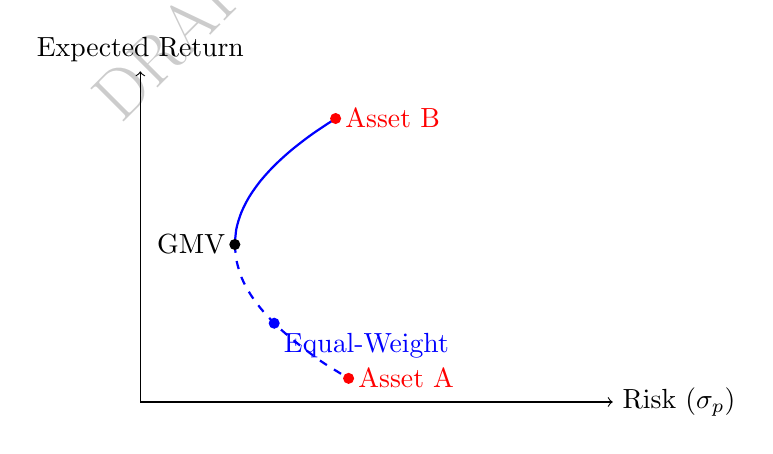
\begin{tikzpicture}[scale=1.0]
        \draw[->] (0,0) -- (6.0,0) node[right] {Risk ($\sigma_p$)};
        \draw[->] (0,0) -- (0,4.2) node[above] {Expected Return};
        \draw[blue,thick,smooth] plot coordinates {(1.2,2.0) (1.22,2.2) (1.28,2.4) (1.38,2.6) (1.52,2.8) (1.7,3.0) (1.92,3.2) (2.18,3.4) (2.48,3.6)};
        \draw[blue,thick,dashed,smooth] plot coordinates {(1.2,2.0) (1.223,1.79) (1.29,1.57) (1.403,1.36) (1.561,1.15) (1.764,0.94) (2.013,0.73) (2.306,0.51) (2.645,0.3)};
        \fill[black] (1.2,2.0) circle (2pt) node[left] {GMV};
        \fill[red] (2.48,3.6) circle (2pt) node[right] {Asset B};
        \fill[red] (2.645,0.3) circle (2pt) node[right] {Asset A};
        \fill[blue] (1.7,1.0) circle (2pt) node[below right] {Equal-Weight};
    \end{tikzpicture}
\end{lrbox}
\ifdim\wd\bookmeasuredbox<0.65\linewidth
\setlength{\bookcapwidth}{0.65\linewidth}
\else
\setlength{\bookcapwidth}{\wd\bookmeasuredbox}
\fi
\ffigbox[\bookcapwidth]{
\usebox{\bookmeasuredbox}
}{
    \caption{A schematic efficient frontier for the two-asset example (solid: efficient; dashed: feasible but dominated). GMV marks the global minimum-variance portfolio, the leftmost attainable point. An investor selects somewhere along the solid segment according to their risk tolerance; GMV is that menu's left endpoint, not its recommended item.}
    \label{fig:efficient_frontier}
}
\end{figure}

Only the upper portion of this curve, starting at the global minimum-variance portfolio and moving toward the higher-returning asset, is efficient in Markowitz's specific sense: every portfolio on this segment offers the highest possible expected return for its level of risk. The lower portion (the dashed segment in Figure~\ref{fig:efficient_frontier}) is feasible, an investor could hold it, but never optimal, since a portfolio directly above it on the efficient segment offers a strictly higher return at the same risk.

It is worth being clear about what the theory does and does not recommend here. The efficient frontier is a menu rather than an answer: the framework narrows the whole feasible region down to that solid upper segment, and the investor then picks a point on it according to how much variance they are willing to bear, a choice the mathematics deliberately leaves open. The global minimum-variance portfolio is simply that menu's left endpoint, the point an investor would choose only if they were unwilling to accept any additional variance whatsoever in exchange for return, so it is better understood as one extreme of the efficient set than as the portfolio the analysis is pointing toward. It nonetheless earns a practical role for a reason that has nothing to do with risk appetite: it is the only point on the frontier whose weights require no expected-return estimates at all, needing only the covariance matrix, which matters a great deal given how badly the estimation-error problem of Section~\ref{sec:matrix-optimization} affects estimated means in particular.

This is the precise, quantitative content behind the informal advice to diversify: it is not merely that diversification feels prudent, but that every portfolio not on the efficient frontier is demonstrably dominated by one that is.

\subsection{Mean-Variance Optimization in Matrix Form}
\label{sec:matrix-optimization}

The two-asset formulas above generalize to any number of assets using matrix notation. For $n$ assets with covariance matrix $\Sigma$ and a vector of ones $\mathbf{1}$, the (unconstrained) global minimum-variance portfolio weights are
\begin{equation*}
w^{\text{MV}} = \frac{\Sigma^{-1}\mathbf{1}}{\mathbf{1}^\top \Sigma^{-1}\mathbf{1}},
\end{equation*}
the direct matrix generalization of the closed-form two-asset formula in Section~\ref{sec:diversification}. Applying this to the three-asset covariance matrix from Chapter 2's AssetA/AssetB/AssetC extension,
\begin{equation*}
\Sigma_3 = \begin{pmatrix} 0.000414 & -0.000198 & -0.000383 \\ -0.000198 & 0.000118 & 0.000176 \\ -0.000383 & 0.000176 & 0.000358 \end{pmatrix},
\end{equation*}
gives minimum-variance weights of
\begin{align*}
w_A &\approx 44.8\%, & w_B &\approx 14.2\%, & w_C &\approx 41.0\%,
\end{align*}
with a portfolio standard deviation of only about $0.050\%$, roughly six times lower than the equal-weighted three-asset portfolio's $0.297\%$ computed in Chapter 2.

This result should be viewed with considerable suspicion rather than celebrated, and the reason is a genuinely important practical lesson.
Chapter 2's three-asset dataset contains only four daily observations, far too few to estimate a $3\times 3$ covariance matrix (six distinct entries) reliably. The matrix-form optimizer above found weights that happen to nearly cancel out the sample's realized co-movements almost perfectly, but it is optimizing against estimation noise as much as against genuine risk, the overfitting\index{overfitting} phenomenon Chapter 6 illustrated with a high-degree polynomial: with enough free parameters relative to the amount of data, a model (here, a portfolio optimizer) can achieve an excellent-looking in-sample result that will not repeat out of sample.
This is widely recognized in practice as Markowitz optimization's central weakness: it is, in Michaud's memorable phrase, an ``estimation-error maximizer,'' since the optimizer actively seeks out and overweights the asset pairs whose historical correlation was most favorable, which are disproportionately likely to be pairs whose favorable correlation was partly a statistical accident of the specific sample rather than a stable underlying relationship.
Sections~\ref{sec:risk-parity} and~\ref{sec:black-litterman} introduce two of the standard practical responses to this problem.

\subsubsection*{Shrinkage Estimation of the Covariance Matrix}\index{covariance shrinkage}
\label{sec:shrinkage}

A direct statistical response to the estimation-error problem above, distinct from the risk parity\index{risk parity} and Black-Litterman approaches developed later in this chapter, is to shrink the noisy sample covariance matrix itself toward a simpler, lower-variance target before ever handing it to the optimizer. A standard target is a diagonal matrix built from the average sample variance, and the shrunk covariance matrix is a weighted average of this target and the raw sample estimate,
\begin{equation*}
\Sigma^{\text{shrunk}} = \delta F + (1-\delta)\Sigma, \qquad F = \bar\sigma^2 I,
\end{equation*}
where $\delta \in [0,1]$ is the shrinkage intensity (often chosen to minimize expected estimation error using a formula due to Ledoit and Wolf, though a fixed value illustrates the idea just as well) and $\bar\sigma^2$ is the average of the sample variances on the diagonal of $\Sigma$. Applying $\delta=0.5$ to the three-asset covariance matrix from Section~\ref{sec:matrix-optimization}, whose average variance is $\bar\sigma^2 \approx 0.000297$, shrinks every off-diagonal covariance term roughly in half and pulls each diagonal variance partway toward the common average. Recomputing the minimum-variance weights using this shrunk covariance matrix gives
\begin{align*}
w_A^{\text{shrunk}} \approx 39.2\%, & & w_B^{\text{shrunk}} \approx 30.5\%, & & w_C^{\text{shrunk}} \approx 30.3\%,
\end{align*}
a far more balanced and intuitively reasonable allocation than the extreme, nearly-single-pair-canceling weights the raw sample covariance matrix produced. The shrunk portfolio's true (sample) variance is necessarily somewhat higher than the unshrunk optimizer's in-sample-minimizing variance, exactly as it must be, since the unshrunk optimizer is defined to be the in-sample minimum by construction; the entire justification for shrinkage is that this modest in-sample cost buys a large improvement in expected out-of-sample reliability, a bias-variance tradeoff directly analogous to the ridge regression penalty Chapter 6 applied to an overfit polynomial.

\section{Equilibrium Models and Factor Approaches}

If everyone optimizes, prices must satisfy conditions of their own; this part develops those conditions and the factor models that relax them.

\subsection{The Capital Asset Pricing Model and Beta Estimation}
\label{sec:capm-beta}

Chapter 5 introduced the Capital Asset Pricing Model, $r_e = r_f + \beta(r_m - r_f)$, to estimate Meridian Fabrication\index{Meridian Fabrication Inc.}'s cost of equity, using an equity beta of $1.2$ that was simply assumed rather than derived. This section closes that gap: beta is, in fact, a regression coefficient, estimated exactly like the OLS regressions of Chapter 6, by regressing an asset's excess returns on the market's excess returns,
\begin{equation*}
r_{i,t} - r_f = \alpha_i + \beta_i (r_{m,t} - r_f) + \varepsilon_t.
\end{equation*}
Table~\ref{tab:capm_data} shows six months of hypothetical excess returns for a stock and the overall market.

\begin{table}[htbp]
\centering
\begin{lrbox}{\bookmeasuredbox}
\begin{tabular}{lrrrrrr}
\toprule
Month & 1 & 2 & 3 & 4 & 5 & 6 \\
Market excess return & $-2.0\%$ & $-1.0\%$ & $0.0\%$ & $1.0\%$ & $2.0\%$ & $3.0\%$ \\
Stock excess return & $-2.5\%$ & $-1.3\%$ & $0.2\%$ & $1.1\%$ & $2.6\%$ & $3.3\%$ \\
\bottomrule
\end{tabular}
\end{lrbox}
\ifdim\wd\bookmeasuredbox<0.65\linewidth
\setlength{\bookcapwidth}{0.65\linewidth}
\else
\setlength{\bookcapwidth}{\wd\bookmeasuredbox}
\fi
\floatbox[\capbot]{table}[\bookcapwidth]{
\usebox{\bookmeasuredbox}
}{
\caption{Six months of excess returns for a stock and the market}
\label{tab:capm_data}
}
\end{table}

Applying the same OLS formulas used throughout Chapter 6,
\begin{equation*}
\hat\beta = \frac{\sum_t (r_{m,t}-\bar r_m)(r_{i,t}-\bar r_i)}{\sum_t (r_{m,t}-\bar r_m)^2} \approx 1.19, \qquad \hat\alpha \approx -0.03\%, \qquad R^2 \approx 0.992.
\end{equation*}
The estimated beta of $1.19$ closely matches the value of $1.2$ that Chapter 5 simply assumed, which is a reassuring, if constructed, confirmation that the earlier chapter's assumption was reasonable, and it illustrates concretely where a CAPM beta actually comes from in practice: not from theory alone, but from a regression identical in form to the ones Chapter 6 introduced for entirely different applications.
The near-zero estimated alpha is also economically meaningful: CAPM predicts that, after accounting for market exposure, no asset should offer a systematically positive or negative excess return, so a statistically significant nonzero alpha (checked using the $t$-statistic and $p$-value machinery introduced in Chapter 6) is often interpreted either as evidence against CAPM or as a genuine mispricing an active manager might try to exploit.

\subsubsection*{Systematic versus Idiosyncratic Risk}\index{Systematic versus Idiosyncratic Risk}

The $R^2 \approx 0.992$ from the regression above has a direct risk-decomposition interpretation, not just a goodness-of-fit one. Total return variance splits into a systematic (market-driven) component and an idiosyncratic (asset-specific) component,
\begin{equation*}
\text{Var}(r_i) = \underbrace{\beta_i^2\,\text{Var}(r_m)}_{\text{systematic}} + \underbrace{\text{Var}(\varepsilon_i)}_{\text{idiosyncratic}},
\end{equation*}
and $R^2$ is the fraction of total variance that is systematic. For the stock in Table~\ref{tab:capm_data}, with returns expressed as decimals, $\text{Var}(r_m) \approx 0.00035$ and systematic variance is $\hat\beta^2\,\text{Var}(r_m) \approx (1.19)^2(0.00035) \approx 0.000494$, against total variance of about $0.000498$, leaving an idiosyncratic remainder of only about $0.0000038$, consistent with the regression's near-perfect fit.

CAPM's central economic claim rests directly on this decomposition: idiosyncratic risk can be diversified away by holding many assets whose asset-specific shocks are independent of one another, the diversification mechanism of Section~\ref{sec:diversification}, so a well-diversified investor should not expect to earn any additional compensation for bearing it.
Systematic risk, by contrast, affects every asset simultaneously through the shared market factor and cannot be diversified away no matter how many assets are added to the portfolio. That is precisely why CAPM's expected-return formula compensates an asset only for its beta (systematic risk) and not for its total volatility. Two assets with identical total volatility but different betas should, under CAPM, offer different expected returns, while two assets with identical betas but very different idiosyncratic volatility should offer the same expected return, a testable and occasionally violated prediction that motivated the multi-factor extensions discussed later in this chapter.

\subsubsection*{The Security Market Line}\index{Security Market Line}

This relationship between beta and expected return has a natural graphical representation, the Security Market Line, plotting CAPM's expected return, $r_f + \beta(r_m-r_f)$, as a straight line against beta itself, shown in Figure~\ref{fig:sml}. Unlike the Capital Market Line of Section~\ref{sec:sharpe-cml} below, which plots return against total risk ($\sigma_p$) and is populated only by efficient portfolios, the Security Market Line plots return against systematic risk (beta) alone and, under CAPM, every correctly priced individual asset or portfolio, efficient or not, should lie exactly on it.

\begin{figure}[htbp]
\centering
\begin{lrbox}{\bookmeasuredbox}
    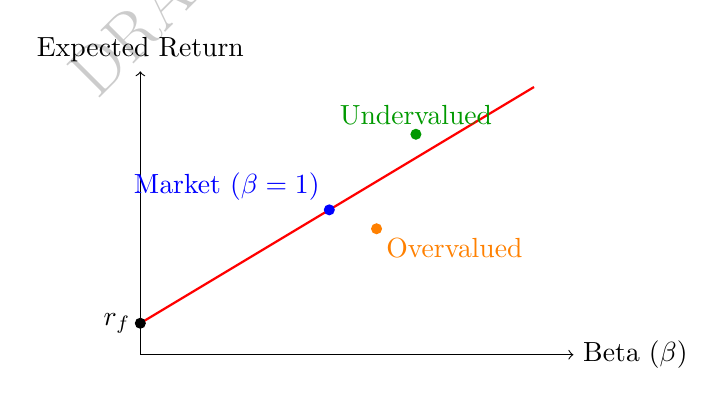
\begin{tikzpicture}[scale=1.0]
        \draw[->] (0,0.6) -- (5.5,0.6) node[right] {Beta ($\beta$)};
        \draw[->] (0,0.6) -- (0,4.2) node[above] {Expected Return};
        \draw[red,thick] (0,1.0) -- (5.0,4.0);
        \fill[black] (0,1.0) circle (2pt) node[left] {$r_f$};
        \fill[blue] (2.4,2.44) circle (2pt) node[above left] {Market ($\beta=1$)};
        \fill[green!60!black] (3.5,3.4) circle (2pt) node[above] {Undervalued};
        \fill[orange] (3.0,2.2) circle (2pt) node[below right] {Overvalued};
    \end{tikzpicture}
\end{lrbox}
\ifdim\wd\bookmeasuredbox<0.65\linewidth
\setlength{\bookcapwidth}{0.65\linewidth}
\else
\setlength{\bookcapwidth}{\wd\bookmeasuredbox}
\fi
\ffigbox[\bookcapwidth]{
\usebox{\bookmeasuredbox}
}{
    \caption{The Security Market Line plots CAPM's expected return against beta, with an undervalued (green) and an overvalued (orange) asset marked relative to it}
    \label{fig:sml}
}
\end{figure}

An asset whose actual expected return plots above the Security Market Line is, under CAPM, undervalued: it offers more expected return than its systematic risk alone would justify, and the nonzero alpha from Section~\ref{sec:capm-beta}'s regression is the vertical distance between an asset's actual position and the line. An asset plotting below the line is correspondingly overvalued.
This is precisely the graphical version of the active-management logic introduced later in this chapter's discussion of the information ratio: an active manager's entire task can be described as searching for assets that plot persistently above the Security Market Line, and a manager who succeeds systematically is finding genuine mispricing rather than simply taking on more systematic risk than their benchmark, which the Security Market Line makes visually explicit in a way that a raw return comparison does not.

\subsection{The Capital Market Line and the Sharpe Ratio}
\label{sec:sharpe-cml}

CAPM's beta measures only one dimension of an asset's risk, its co-movement with the market; the Sharpe ratio\index{Sharpe ratio} provides a complementary, portfolio-level summary of risk-adjusted performance,
\begin{equation*}
\text{Sharpe Ratio} = \frac{\bar r_p - r_f}{\sigma_p},
\end{equation*}
the excess return earned per unit of total risk taken. Comparing the equal-weighted and minimum-variance two-asset portfolios from Section~\ref{sec:diversification}, using their sample mean returns of $0.88\%$ and $0.92\%$ respectively and treating the daily risk-free rate as approximately zero for this short-horizon illustration,
\begin{equation*}
\text{Sharpe}_{\text{equal}} = \frac{0.88\%}{0.583\%} \approx 1.51, \qquad \text{Sharpe}_{\text{MV}} = \frac{0.92\%}{0.322\%} \approx 2.85.
\end{equation*}
The minimum-variance portfolio not only has lower risk, as expected by construction, but also a substantially higher Sharpe ratio, since it happens to also have a slightly higher mean return in this particular sample; this is not a general guarantee (the minimum-variance portfolio does not target return at all) but is a useful reminder that lower risk and competitive returns are not mutually exclusive.

Plotting every portfolio's Sharpe ratio against a combination of the risk-free asset and the tangency portfolio (the portfolio of risky assets with the single highest Sharpe ratio) produces the Capital Market Line, illustrated in Figure~\ref{fig:cml}, the set of risk-return combinations achievable by mixing the risk-free asset with that one specific risky portfolio.

\begin{figure}[htbp]
\centering
\begin{lrbox}{\bookmeasuredbox}
    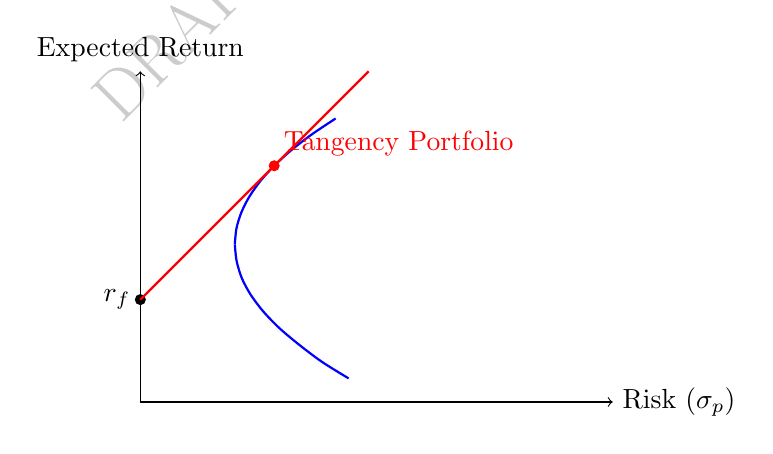
\begin{tikzpicture}[scale=1.0]
        \draw[->] (0,0) -- (6.0,0) node[right] {Risk ($\sigma_p$)};
        \draw[->] (0,0) -- (0,4.2) node[above] {Expected Return};
        \draw[blue,thick,smooth] plot coordinates {(1.2,2.0) (1.223,1.79) (1.29,1.57) (1.403,1.36) (1.561,1.15) (1.764,0.94) (2.013,0.73) (2.306,0.51) (2.645,0.3)};
        \draw[blue,thick,smooth] plot coordinates {(1.2,2.0) (1.22,2.2) (1.28,2.4) (1.38,2.6) (1.52,2.8) (1.7,3.0) (1.92,3.2) (2.18,3.4) (2.48,3.6)};
        \fill[black] (0,1.3) circle (2pt) node[left] {$r_f$};
        \draw[red,thick] (0,1.3) -- (2.9,4.2);
        \fill[red] (1.7,3.0) circle (2pt) node[above right] {Tangency Portfolio};
    \end{tikzpicture}
\end{lrbox}
\ifdim\wd\bookmeasuredbox<0.65\linewidth
\setlength{\bookcapwidth}{0.65\linewidth}
\else
\setlength{\bookcapwidth}{\wd\bookmeasuredbox}
\fi
\ffigbox[\bookcapwidth]{
\usebox{\bookmeasuredbox}
}{
    \caption{The Capital Market Line (red) is tangent to the efficient frontier of risky assets (blue) at the tangency portfolio}
    \label{fig:cml}
}
\end{figure}

A central result of modern portfolio theory (the two-fund separation theorem\index{two-fund separation theorem}) is that every investor, regardless of their individual risk tolerance, should hold some combination of only the risk-free asset and this single tangency portfolio, differing only in how much of each they hold, not in the composition of the risky portion itself.
A more risk-averse investor simply holds more of the risk-free asset and less of the tangency portfolio, while a less risk-averse investor may even borrow at the risk-free rate to hold more than $100\%$ of their wealth in the tangency portfolio, moving further out along the Capital Market Line in either direction without ever needing to change which risky assets they hold or in what proportion.

\subsubsection*{A Worked Example: Computing the Tangency Portfolio}\index{Tangency Portfolio}
\label{sec:tangency-portfolio}

The tangency portfolio pictured in Figure~\ref{fig:cml} has a closed-form solution directly analogous to the minimum-variance formula of Section~\ref{sec:diversification}, maximizing the Sharpe ratio rather than minimizing variance alone,
\begin{equation*}
w^{\text{tan}} = \frac{\Sigma^{-1}(\boldsymbol{\mu}-r_f\mathbf{1})}{\mathbf{1}^\top\Sigma^{-1}(\boldsymbol{\mu}-r_f\mathbf{1})},
\end{equation*}
the matrix generalization of maximizing $(\bar r_p - r_f)/\sigma_p$ directly rather than minimizing $\sigma_p^2$ alone. Applying this to AssetA and AssetB, with mean daily returns $\mu_A=0.76\%$, $\mu_B=1.00\%$ and, as in Section~\ref{sec:sharpe-cml}'s Sharpe ratio calculation above, a risk-free rate of approximately zero for this short-horizon illustration, gives
\begin{align*}
w_A^{\text{tan}} &= 33.76\%, & w_B^{\text{tan}} &= 66.24\%,
\end{align*}
strikingly close to the minimum-variance weights of $34.05\%$ and $65.95\%$ computed in Section~\ref{sec:diversification}, with a Sharpe ratio of $2.849$, barely above the minimum-variance portfolio's own $2.848$.

This near-coincidence is specific to this dataset, not a general property of the tangency portfolio, and it is worth seeing a case where the two portfolios genuinely differ to understand why.
With $r_f\approx 0$ and both assets' mean returns small relative to their risk, the excess-return vector $\boldsymbol\mu - r_f\mathbf{1}$ that drives the tangency formula is nearly proportional to a constant vector, which makes $w^{\text{tan}}$ collapse close to the minimum-variance weights (driven purely by $\Sigma^{-1}\mathbf{1}$) almost by coincidence. Applying the identical formula to Section~\ref{sec:robo-advisors}'s equity/bond assumptions instead ($\sigma_e=16\%$, $\sigma_b=5\%$, $\rho_{eb}=-0.20$, $r_e=8\%$, $r_b=3\%$), with a more economically meaningful risk-free rate of $r_f=2\%$, gives a tangency portfolio of
\begin{align*}
w_e^{\text{tan}} &= 32.0\% \text{ equities}, & w_b^{\text{tan}} &= 68.0\% \text{ bonds}, & \text{Sharpe} &= 0.468,
\end{align*}
meaningfully different from that section's minimum-variance weights of $13.1\%$ equities and $86.9\%$ bonds (Sharpe ratio $0.374$ at the same risk-free rate). The lesson generalizes: the tangency portfolio and the minimum-variance portfolio coincide only when expected returns happen not to matter much for distinguishing one asset from another relative to their risk; whenever expected returns differ meaningfully across assets, as equities and bonds do here, the two portfolios can diverge substantially, and only the tangency portfolio is actually the one the two-fund separation theorem recommends every investor hold in combination with the risk-free asset.

\subsection{Multi-Factor Models: Beyond a Single Market Beta}
\label{sec:factor-models}

CAPM's single market factor, while foundational, leaves systematic patterns in average returns unexplained; empirically, smaller companies and companies with high book-to-market ratios have historically earned higher average returns than CAPM's single beta predicts. Fama and French's three-factor model\index{Fama-French three-factor model} extends CAPM by adding two additional factors, SMB (Small Minus Big, the return of small-capitalization stocks minus large-capitalization stocks) and HML (High Minus Low, the return of high book-to-market ``value'' stocks minus low book-to-market ``growth'' stocks), on top of the original market factor:
\begin{equation*}
r_{i,t} - r_f = \alpha_i + \beta_{i,\text{MKT}}(r_{m,t}-r_f) + \beta_{i,\text{SMB}}\,\text{SMB}_t + \beta_{i,\text{HML}}\,\text{HML}_t + \varepsilon_t.
\end{equation*}
Estimating a two-factor version of this model (market and SMB only, for a compact illustration) requires the matrix form of OLS introduced conceptually in Chapter 6, $\hat\beta = (X^\top X)^{-1}X^\top y$, since more than one explanatory variable no longer admits the simple single-variable formulas used earlier in this chapter. Fitting this to six months of hypothetical market, SMB, and asset return data gives
\begin{align*}
\hat\alpha &\approx -0.6\%, & \hat\beta_{\text{MKT}} &\approx 1.19, & \hat\beta_{\text{SMB}} &\approx 0.35, & R^2 &\approx 0.999;
\end{align*}
the positive SMB loading indicates the asset behaves somewhat like a small-cap stock, earning a return premium associated with that factor beyond what its market beta alone would predict.

Each additional factor in a model like this is, in effect, an additional explanatory variable in a multiple regression, so the model-selection and overfitting cautions from Chapter 6 apply directly. Adding enough factors will always improve in-sample $R^2$. That is why serious factor-model research relies on economically motivated factors validated out of sample, rather than a large, undisciplined search over every conceivable candidate factor, a practice sometimes derided in the finance literature as data mining for a ``factor zoo.''

Multi-factor models have moved from academic research into everyday investment products through so-called ``smart beta'' or factor-based exchange-traded funds. These construct a portfolio designed to have deliberately high exposure to a specific factor, such as value, size, momentum, or low volatility, rather than simply weighting holdings by market capitalization as a traditional index fund does.
The appeal of these products is direct: if a factor like SMB or HML has historically earned a return premium, an investor may prefer to capture that premium systematically and at low cost through a rules-based fund rather than paying an active manager to attempt the same thing through discretionary stock selection.
The same overfitting caution above applies with particular force here, since a factor's historical premium, discovered through the kind of statistical search this section warns against, can weaken or disappear once it becomes widely known and systematically invested in, as more capital chasing the same factor exposure competes away the very mispricing the premium was compensating for, a dynamic with a direct analogue in Chapter 3's discussion of market efficiency: a genuinely exploitable pattern tends not to remain exploitable once it is discovered and traded on at scale.

\subsection{Risk Parity: A Correlation-Light Alternative}
\label{sec:risk-parity}

Section~\ref{sec:matrix-optimization} showed that full mean-variance optimization can be dangerously sensitive to estimation error in the covariance matrix, particularly its off-diagonal correlation terms, which are typically the hardest entries to estimate precisely. Risk parity sidesteps much of this fragility by allocating weight inversely to volatility alone, ignoring correlation entirely,
\begin{equation*}
w_i^{\text{RP}} = \frac{1/\sigma_i}{\sum_j 1/\sigma_j}.
\end{equation*}
Applied to AssetA and AssetB,
\begin{align*}
w_A^{\text{RP}} &= 34.8\%, & w_B^{\text{RP}} &= 65.2\%, & \text{Sharpe} &\approx 2.84,
\end{align*}
remarkably close to the true minimum-variance weights of $34.1\%$ and $65.9\%$ (Sharpe ratio $2.85$) computed in Section~\ref{sec:diversification} despite using far less information (no correlation estimate at all).
This is not a coincidence specific to this dataset: when volatilities differ substantially more than correlations do, as is common across many real asset classes, inverse-volatility weighting is a robust approximation to the mean-variance optimum that requires estimating only $n$ volatilities rather than the full $n(n-1)/2$ correlation pairs, each of which is an additional source of estimation error of the kind that made the three-asset optimization in Section~\ref{sec:matrix-optimization} so unreliable.
This tradeoff, accepting a method that is provably suboptimal under the classical theory's own assumptions in exchange for far greater robustness to violations of those assumptions, is a recurring and important theme in practical portfolio management.

\subsection{Black-Litterman: Blending Views with Market Equilibrium}
\label{sec:black-litterman}

Suppose you manage the $60/40$ portfolio of Section~\ref{sec:sixty-forty} and you come to work with exactly one opinion: equities look cheap relative to bonds. This is the ordinary situation of a working investor, and it is one the optimizer of Section~\ref{sec:matrix-optimization} simply cannot accept. That machinery demands a complete vector of expected returns, one number for every asset in the portfolio, so before it will run at all you must also hand it an expected return for bonds, about which you have no opinion whatsoever. Whatever number you invent, the optimizer treats it as a firmly held belief and acts on it exactly as decisively as on the view you actually hold.

There is a second problem, and it is just as practical. The formula has nowhere to record how sure you are. An opinion you would stake your reputation on and one you formed over coffee enter the calculation identically and produce identical portfolios, even though the difference between them is precisely what ought to determine how far the portfolio moves away from where it started.

Both problems land on the input that can least afford them. Chopra and Ziemba quantified this directly: for a typical investor's risk tolerance, errors in estimated \emph{means} are roughly an order of magnitude more costly, in terms of the utility actually lost, than errors of the same relative size in variances, which are in turn about twice as costly as errors in covariances. The expected-return vector is the most fragile input in the entire apparatus, and the na\"ive procedure requires you to fabricate most of it in order to express one genuine view. That same ordering is why the global minimum-variance portfolio of Section~\ref{sec:efficient-frontier} is more robust than its position at one extreme of the efficient frontier would suggest: needing no expected returns at all, it is immune to the largest error source by construction.

The Black-Litterman model answers both objections at once, and it does so without touching the covariance matrix. It supplies a default answer to ``what do I think about bonds?'' so that holding no opinion becomes a position the mathematics can actually represent, and it lets every opinion you do hold carry an explicit statement of how confident you are in it.

The default comes from the market itself. Other investors' collective holdings are observable, and if those holdings are broadly sensible then they already encode a set of expected returns: whatever numbers would have made that particular portfolio the optimal one to hold. Recovering them means running Section~\ref{sec:matrix-optimization}'s machinery backward, a step called reverse optimization\index{reverse optimization}, which deduces the excess returns $\boldsymbol\Pi$ that make the observed market weights $w_{\text{mkt}}$ optimal instead of deducing weights from returns,
\begin{equation*}
\boldsymbol\Pi = \delta\,\Sigma\,w_{\text{mkt}},
\end{equation*}
where $\delta$ is the market's coefficient of risk aversion. This is the answer to the bond question: not a number you made up, but the one implied by what everyone else is already doing.

Your own opinions then enter through three objects, each corresponding to something an investor can actually say. A matrix $P$ records which assets each view is about, so that ``equities relative to bonds'' can be expressed without saying anything about either one on its own. A vector $Q$ gives the magnitudes claimed. And a matrix $\Omega$ states, on its diagonal, how uncertain each view is, which is where ``I would stake my reputation on this'' and ``this is a hunch'' finally become different inputs. The blend of prior and views is then
\begin{equation*}
E[R] = \left[(\tau\Sigma)^{-1} + P^\top\Omega^{-1}P\right]^{-1}\left[(\tau\Sigma)^{-1}\boldsymbol\Pi + P^\top\Omega^{-1}Q\right],
\end{equation*}
the scalar $\tau$ setting how tightly the equilibrium prior itself is held. Intimidating as the notation looks, it is doing something familiar: this is Chapter 1's Bayesian update written in matrix form, with $\boldsymbol\Pi$ as the prior, $Q$ as the evidence, and $\Omega^{-1}$ as the weight that evidence earns. A confident view (small $\Omega$) pulls the answer toward $Q$; a tentative one leaves it near $\boldsymbol\Pi$.

The two consequences are worth stating plainly, because they are exactly what the opening two problems asked for. An investor with no views at all gets the market weights back, unchanged, so ``I have no opinion'' now produces a sensible portfolio rather than an arbitrary one. And an investor with a view, such as ``I believe equities will outperform bonds by 9\% over the coming year,'' gets a portfolio tilted away from the market by an amount that depends on how firmly the view was asserted, rather than the unconstrained lurch a purely historical-return optimizer would deliver. This is what makes Black-Litterman well suited to combining a systematic, data-driven baseline with the qualitative, analyst-driven judgment that a purely statistical model like those in Chapter 6 cannot generate on its own. The worked example that follows shows both consequences as numbers.

\subsection{A Worked Example: Blending a View into a 60/40 Portfolio}\index{Black-Litterman model}
\label{sec:bl-example}

Take the equity and bond assumptions Section~\ref{sec:tangency-portfolio} already used ($\sigma_e=16\%$, $\sigma_b=5\%$, $\rho_{eb}=-0.20$, $r_f=2\%$) and treat Section~\ref{sec:sixty-forty}'s classic $60/40$ split as the market portfolio. That portfolio's volatility is $9.41\%$ and, under the same $8\%$ and $3\%$ expected returns, its excess return is $4.00\%$, which pins down the risk-aversion coefficient as $\delta = 0.0400/0.0941^2 = 4.52$. Reverse optimization then implies equilibrium excess returns of
\begin{align*}
\Pi_e &= 6.6546\%, & \Pi_b &= 0.0181\%.
\end{align*}
Two features of this prior deserve attention before any view is added. These are not the $8\%$ and $3\%$ assumed a moment ago, and they were never meant to be: they are the returns that would make a $60/40$ investor's weights optimal, so the implied equity-minus-bond spread, $6.6546\% - 0.0181\% = 6.6365\%$, is simply wider than the $5.00\%$ those assumptions embed. Bonds, meanwhile, earn almost no equilibrium premium at all, which is not a claim that bonds are unattractive but a consequence of their low volatility and negative correlation contributing almost nothing to the $60/40$ portfolio's total risk, precisely what a risk-based equilibrium ought to conclude.

Now suppose the investor holds the single view quoted above, that equities will beat bonds by $9\%$, against the $6.6365\%$ equilibrium already implies. Setting $P = (1, -1)$, $Q = 9\%$, $\tau = 0.05$, and $\Omega = P(\tau\Sigma)P^\top$, which calibrates the view's uncertainty to the prior's own uncertainty about that same spread, the posterior expected excess returns become $7.68\%$ for equities and $-0.14\%$ for bonds, and the resulting optimal weights are
\begin{align*}
w_e &= 68.4\% \text{ equities}, & w_b &= 31.6\% \text{ bonds}.
\end{align*}
The view moved the portfolio $8.4$ percentage points toward equities rather than to a corner, and the size of that move tracks the confidence attached to it: halving $\Omega$, which asserts the view more firmly, produces $71.1/28.9$, while tripling it produces only $64.2/35.8$. That bounded, monotone response is the entire point of the construction. The same $9\%$ opinion yields a tilt the investor can dial rather than the violent swing a purely historical-return optimizer would produce from identical information, and setting the view aside altogether returns exactly $60/40$, the equilibrium the model began from.

\section{Building and Running a Portfolio}

A portfolio on paper becomes a portfolio in practice only after constraints, costs, currencies, and mandates are imposed on it.

\subsubsection*{Practical Allocation Decisions: Constraints, Rebalancing, and Transaction Costs}

The mathematical portfolios developed so far in this chapter ignore several frictions that matter enormously in practice. Real portfolios are usually subject to constraints beyond the mathematics of the optimization itself: a long-only mandate prohibits negative weights (short positions), which the unconstrained formulas in Sections~\ref{sec:diversification} and~\ref{sec:matrix-optimization} do not rule out on their own, and position limits or sector caps may further restrict how concentrated any single holding or sector can become, both of which typically require solving the optimization as a constrained quadratic program rather than using the closed-form matrix formulas presented above.

A concrete example shows exactly when this constraint binds. Consider two assets with $\sigma_X=8\%$, $\sigma_Y=20\%$, and an unusually high correlation of $\rho_{XY}=0.9$. Applying the closed-form minimum-variance formula from Section~\ref{sec:diversification} gives
\begin{align*}
w_X^{\text{MV}} &\approx 145.5\%, & w_Y^{\text{MV}} &\approx -45.5\%, & \sigma_p &\approx 5.26\%,
\end{align*}
a substantial short position in Asset Y financing a leveraged long position in Asset X, achieving an unconstrained portfolio volatility below either individual asset's own volatility. A long-only mandate rules this out entirely, and because portfolio variance is monotonically decreasing in $w_X$ across the entire feasible range $w_X \in [0,1]$ on the way toward the (infeasible) unconstrained optimum, the best achievable long-only portfolio is the corner solution $w_X=100\%$, $w_Y=0\%$, with volatility equal to Asset X's own $8\%$.
In this particular case, the long-only constraint does not merely reduce the benefit of diversification; it eliminates it completely, since every feasible long-only combination of the two assets is riskier than holding Asset X alone. This is a direct illustration of why the unconstrained formulas developed earlier in this chapter are a starting point for intuition rather than a literal prescription: real portfolio construction almost always requires solving a constrained optimization problem numerically, and the constraints themselves can qualitatively change the character of the optimal solution, not just its exact numerical weights.

Even a well-constructed portfolio does not stay at its target weights on its own, since different assets earn different returns over time and weights drift accordingly, so rebalancing back to target weights is periodically necessary. Every rebalancing trade, however, incurs the transaction costs introduced in Chapter 3, including at least half the bid-ask spread\index{bid-ask spread} and any market impact\index{market impact} from the trade's size, so frequent rebalancing that chases small deviations from target weights can destroy more value in trading costs than it preserves in risk control.

Consider a \$1,000,000 portfolio that has drifted 5 percentage points from its target weights, requiring a \$50,000 trade in each direction (selling the overweight asset, buying the underweight one) to restore them. At a one-way transaction cost of 15 basis points, roughly consistent with the bid-ask-spread-based costs introduced in Chapter 3, each \$50,000 trade costs $\$50{,}000 \times 0.0015 = \$75$, for a total round-trip rebalancing cost of $\$150$, or $0.015\%$ of the portfolio's value. This may look negligible for a single rebalancing event. But a manager who rebalances daily in response to every small drift compounds this cost across hundreds of trading days per year. That is precisely why practitioners typically rebalance on a fixed calendar schedule, quarterly for example, or only once a weight has drifted beyond some tolerance band, rather than continuously. The choice explicitly trades off tracking the target allocation precisely against the cumulative transaction-cost drag of doing so too often.

Taxable investors face a further consideration entirely absent from the mathematics above: selling an appreciated position to rebalance can trigger a capital gains tax liability, so a tax-aware rebalancing strategy may deliberately tolerate more allocation drift than the pure risk-minimization mathematics would recommend, in exchange for deferring a tax cost.

\subsection{Solving the Constrained Problem Numerically}
\label{sec:constrained-optimization}

Once inequality constraints such as a long-only mandate or a position cap are added, the elegant closed-form matrix formulas of Sections~\ref{sec:diversification} and~\ref{sec:matrix-optimization} no longer apply directly, since those formulas were derived by setting a gradient to zero, a technique that only characterizes an unconstrained (or purely equality-constrained) optimum. The general constrained minimum-variance problem is instead stated and solved as
\begin{equation*}
\min_{\bf w}\; {\bf w}^\top \Sigma\, {\bf w} \quad \text{subject to} \quad {\bf w}^\top \mathbf{1} = 1, \quad {\bf w}^\top \boldsymbol{\mu} = r_0 \;\text{(optional)}, \quad w_i^{\text{low}} \le w_i \le w_i^{\text{high}} \;\; \forall i,
\end{equation*}
where the budget constraint (${\bf w}^\top\mathbf{1}=1$) is always present, the target-return constraint is included only when tracing a specific point on the efficient frontier rather than the global minimum-variance portfolio itself, and the box constraint $w_i^{\text{low}}=0$, $w_i^{\text{high}}=1$ recovers a long-only mandate, a tighter $w_i^{\text{high}}$ recovers a position or sector cap, and $w_i^{\text{low}} < 0$ permits limited short selling.

This is a quadratic objective with linear constraints, solved in practice with a numerical constrained optimizer, most commonly sequential quadratic programming (SLSQP), available directly as \texttt{scipy.\allowbreak optimize.\allowbreak minimize(..., method="SLSQP")} in Python, which iterates toward a solution rather than computing one in a single matrix step the way Sections~\ref{sec:diversification} and~\ref{sec:matrix-optimization}'s formulas do.

Applying this numerical approach to the AssetX/AssetY example above, minimizing variance subject to the budget constraint and long-only bounds $0 \le w_i \le 1$, converges in a handful of iterations to $w_X = 100\%$, $w_Y = 0\%$, the corner solution derived by hand above, a useful confidence check that the numerical method and the closed-form reasoning agree exactly where both are available.

One practical wrinkle is worth flagging explicitly, since it is easy to miss: a generic optimizer's default convergence tolerance is tuned for objective values of a typical order of magnitude, and the raw portfolio variances in this chapter, on the order of $0.0001$ or smaller for daily returns, are small enough that a naive call can terminate after a single iteration at whatever starting point was supplied, silently reporting success despite having barely moved. Rescaling the objective, for instance by working in squared-percent units rather than raw squared decimals, or tightening the optimizer's tolerance explicitly, avoids this failure mode; the companion notebook shows both the failure and the fix side by side.

This machinery also makes it possible to revisit Section~\ref{sec:matrix-optimization}'s three-asset minimum-variance portfolio (weights of $44.8\%$, $14.2\%$, and $41.0\%$ in AssetA, AssetB, and AssetC, with a volatility of about $0.050\%$) under a position cap no single asset may exceed, a common institutional constraint that the closed-form formula cannot express at all. Capping every weight at $40\%$ forces AssetA's allocation down from its unconstrained $44.8\%$ to the $40\%$ cap, with the freed-up weight redistributed to the other two assets:
\begin{align*}
w_A^{\text{cap}} &= 40.0\%, & w_B^{\text{cap}} &= 28.4\%, & w_C^{\text{cap}} &= 31.6\%, & \sigma_p^{\text{cap}} &\approx 0.113\%,
\end{align*}
more than double the uncapped minimum-variance portfolio's $0.050\%$, a concrete price paid for the diversification-forcing discipline the cap imposes.

Tracing out a full constrained efficient frontier under the same $40\%$ cap follows the same recipe with the optional target-return constraint included: solving for the minimum-variance portfolio achieving a $0.75\%$ expected return, for instance, gives
\begin{align*}
w_A &= 40.0\%, & w_B &= 35.1\%, & w_C &= 24.9\%, & \sigma_p &\approx 0.136\%,
\end{align*}
one point on a constrained frontier that a reader can trace fully by sweeping the target return $r_0$ across a grid and re-solving at each point, exactly as the companion notebook does.

\subsection{Tracking Error and the Information Ratio}
\label{sec:tracking-error}

Many portfolio managers are evaluated not on absolute return alone but relative to a specified benchmark, and the Sharpe ratio of Section~\ref{sec:sharpe-cml} has a direct benchmark-relative analogue. The active return in any period is simply the portfolio's return minus the benchmark's return, $r_t^{\text{active}} = r_t^p - r_t^b$, and tracking error is the standard deviation of this active return series,
\begin{equation*}
\text{Tracking Error} = \text{std}(r^{\text{active}}).
\end{equation*}
Using Chapter 2's equal-weighted AssetA/AssetB portfolio returns as the ``portfolio'' and AssetB's own returns as a hypothetical benchmark, the active returns across the four days are
\begin{align*}
r_1^{\text{active}} &= 0.50\%, & r_2^{\text{active}} &= -1.24\%, & r_3^{\text{active}} &= 1.74\%, & r_4^{\text{active}} &= -1.48\%,
\end{align*}
giving a tracking error of $1.52\%$ and a mean active return of $-0.12\%$. The information ratio, the active-return analogue of the Sharpe ratio, divides the two,
\begin{equation*}
\text{Information Ratio} = \frac{\text{mean active return}}{\text{Tracking Error}} \approx \frac{-0.12\%}{1.52\%} \approx -0.08,
\end{equation*}
a small negative value indicating that, over this short and deliberately illustrative sample, the portfolio slightly underperformed its benchmark per unit of active risk taken. This is the kind of number a manager and their client would examine closely. A persistently negative information ratio suggests a manager is not adding value relative to simply holding the benchmark, net of whatever fees the active management arrangement costs. A positive and statistically significant one (again checked with the same $t$-statistic machinery from Chapter 6) is one standard piece of evidence that a manager's active decisions are genuinely adding value rather than reflecting noise.

\subsubsection*{Machine Learning in Portfolio Construction}
\label{sec:ml-portfolio}

The classical methods in this chapter estimate their inputs, expected returns, variances, and covariances, using simple sample statistics, but every one of those inputs is itself a prediction problem that the machine learning methods of Chapter 6 can potentially improve. Regularized regression (ridge or LASSO, introduced in Chapter 6's discussion of overfitting) can estimate expected returns or factor exposures more stably than raw historical averages, shrinking noisy coefficient estimates toward zero in a manner directly analogous to the covariance shrinkage of Section~\ref{sec:shrinkage}.

\subsection{Can Machine Learning Forecast Expected Returns?}\index{return predictability}
\label{sec:ml-expected-returns}

Section~\ref{sec:black-litterman} established that expected returns are the input whose estimation errors cost the most, so the obvious question is whether the methods of Chapter 6 can predict them better than a historical average can. This has been tested about as thoroughly as any question in empirical finance. Gu, Kelly, and Xiu ran the full comparison, putting ordinary least squares, penalized linear models, random forests, gradient-boosted trees, and neural networks on the same footing across roughly thirty thousand US stocks and ninety-four firm characteristics over six decades. Neural networks and tree ensembles won clearly, for the same reason they won in Section~\ref{sec:ml-factor-ridge}'s much smaller example, namely their ability to capture interactions and nonlinearities that a linear specification cannot represent, and the linear benchmarks were close to useless out of sample.

The headline result is a monthly out-of-sample $R^2$ of roughly $0.40\%$, and a reader arriving from Chapter 6 will read that as a catastrophic failure. It is not, and understanding why is the most transferable lesson in this section. Monthly equity volatility runs around $5\%$ against an expected return near $0.7\%$, so noise genuinely dominates signal by construction, and an $R^2$ near half a percent sits close to what is attainable rather than far below it. Campbell and Thompson made the argument precise: the right yardstick for a return forecast is not the fraction of variance it explains but the squared Sharpe ratio of the portfolio it funds, and by that standard a monthly $R^2$ of half a percent is economically substantial. Gu, Kelly, and Xiu's long-short portfolios formed on the neural-network forecasts duly earned Sharpe ratios far above what their linear competitors managed.

Three features of the problem keep it hard, and none of them will be familiar from a standard machine learning course. The signal-to-noise ratio, as just described, is a property of the phenomenon rather than of the estimator. The target is adaptive and, in effect, adversarial: McLean and Pontiff found that documented anomaly returns shrink by roughly a quarter between a study's sample period and the period immediately after it, and by well over half once the result is published, which is to say that a pattern degrades precisely because someone found it. And the data are scarcer than they look, since sixty years of monthly observations amount to only a few hundred points per series, a thin diet for a method designed for millions of images.

Putting this beside Section~\ref{sec:black-litterman}'s ordering yields the uncomfortable summary of this whole chapter's estimation problem: predictability runs in the opposite direction from importance. Variances and covariances, whose errors cost the least, are the most forecastable, which is why the volatility models of Chapter 7 work as well as they do. The level of expected returns, whose errors cost the most, is the least forecastable. In between sits cross-sectional prediction, deciding which assets will outperform which, which is materially more tractable than predicting the market's direction and is where nearly all of the successful applied work concentrates.

This also settles where an ML forecast should enter a portfolio process. Feeding it directly into Section~\ref{sec:matrix-optimization}'s optimizer as $\boldsymbol\mu$ discards the one thing that makes it usable, which is that the model reports not only a prediction but the accuracy of its own past predictions. A model that emits a forecast together with an out-of-sample error is producing the pair Black-Litterman asks for, a view $Q$ and its uncertainty $\Omega$, and routing it that way makes the resulting tilt automatically proportional to how much the model has actually earned. A predictor with a $0.40\%$ $R^2$ receives a correspondingly large $\Omega$ and moves the portfolio only slightly, which is the correct response to a weak but genuine signal rather than a disappointment.

\subsection{A Head-to-Head Test: Ridge Regression versus OLS on Collinear Factors}\index{Ridge regression for factor exposures}
\label{sec:ml-factor-ridge}

Section~\ref{sec:factor-models}'s two-factor example uses only six months of data and two clearly distinct factors, too clean a setting to show a genuine estimation-error problem. A real factor library is rarely this well-behaved: candidate factors are often correlated with one another, momentum and a ``quality'' factor both partly reflect recent price strength, say, and a short history makes that collinearity far more damaging.
The companion notebook extends the factor regression to twelve months and five candidate factors (market, SMB, HML, momentum, and quality), with quality \emph{constructed} as a near-linear combination of HML and momentum ($0.61$ and $0.89$ correlation respectively) to mimic this real-world redundancy, and with known true exposures $\beta=(1.10, 0.30, 0.20, -0.10, 0.15)$ so that each estimator's error can be measured directly against ground truth rather than only against a single sample's noisy realized returns.

Ordinary least squares, fit on all twelve months, badly overfits this short, collinear history:
\begin{align*}
\hat\beta_{\text{OLS}} &= (1.078,\ -0.467,\ 0.979,\ 1.435,\ -2.322), & \text{RMSE} &= 1.390,
\end{align*}
getting the market exposure roughly right but the SMB sign backward, wildly overstating HML and momentum, and estimating a quality exposure of $-2.322$ against a true value of $+0.15$, an error of more than two and a half units on a coefficient that should be modest. A ridge regression fit on the identical data, with a shrinkage penalty chosen to be small but nonzero, instead recovers
\begin{align*}
\hat\beta_{\text{ridge}} &= (0.957,\ 0.124,\ 0.027,\ -0.011,\ -0.075), & \text{RMSE} &= 0.167,
\end{align*}
still imperfect, but with every coefficient pulled back toward a plausible order of magnitude and no wild sign reversal on a factor that should matter, an $88\%$ RMSE reduction against the five true exposures. This mirrors almost exactly the covariance-shrinkage story of Section~\ref{sec:shrinkage}. The raw, unregularized estimator is not simply less precise but actively misleading, fitting the specific collinear noise pattern this one short sample happened to contain, while a modest shrinkage penalty trades a small amount of bias for a large reduction in this kind of estimation-error blowup.

Clustering methods, such as the $K$-means algorithm Chapter 6 applied to group firms by leverage and profit margin, can be applied instead to group assets by return co-movement before optimizing, an approach known as hierarchical risk parity\index{Hierarchical Risk Parity}: rather than inverting a single, potentially ill-conditioned covariance matrix across all assets simultaneously (the source of the estimation-error fragility in Section~\ref{sec:matrix-optimization}), the portfolio is built recursively, first allocating risk across clusters of similar assets and then within each cluster.
This tends to produce allocations that are more stable and diversified than na\"ive full-matrix mean-variance optimization when the number of assets is large relative to the length of the available return history.

More recent research has extended tree-based ensembles and neural networks (both introduced in Chapter 6) directly to return prediction and portfolio weight generation, training a model to output portfolio weights that maximize a risk-adjusted objective like the Sharpe ratio directly, rather than first predicting returns and then feeding those predictions into a separate mean-variance optimization step.
This end-to-end approach can, in principle, avoid compounding two separate sources of error (prediction error and optimization error), but it inherits every overfitting and interpretability concern Chapter 6 raised, in a setting where an opaque, poorly validated model directly controls real capital allocation, the model risk management\index{model risk management} concerns Chapter 8 discussed at length. As in every other application of machine learning to finance covered in this book, the message is not that these methods should be avoided, but that they must be validated, monitored, and understood by the people ultimately responsible for the capital they allocate, not deployed simply because they are available.

A further, more experimental line of research frames the entire allocation and rebalancing decision as a sequential decision-making problem and applies reinforcement learning, an approach in which an algorithm learns a trading or allocation policy directly through simulated trial and error against a reward signal such as risk-adjusted return net of transaction costs, rather than through a single-shot prediction and optimization step.
This framing is naturally suited to the rebalancing tradeoffs discussed later in this chapter, since a reinforcement learning agent can, in principle, learn to weigh the benefit of tracking target weights closely against the transaction-cost drag of trading too frequently within a single unified objective, rather than treating rebalancing policy and portfolio construction as two separate decisions.
The same caution applies here with even greater force: a reinforcement learning agent trained in a simulated market environment inherits every assumption baked into that simulation, and a policy that performs well in simulation can fail unpredictably when deployed against real markets whose dynamics differ from the training environment in ways that were never anticipated, an especially acute version of the non-stationarity concern raised throughout this book.

\subsubsection*{International Diversification and Currency Risk}
\label{sec:international-diversification}

Every example so far in this chapter has implicitly assumed a single currency, but a portfolio that holds foreign assets introduces an additional risk factor absent from the domestic case: currency risk, the risk that movements in exchange rates change the domestic-currency value of a foreign holding independently of how that asset performs in its own local market.
A US investor holding a European stock earns a return that combines the stock's local-currency performance with the euro's movement against the dollar over the same period, and these two components can partially offset or reinforce each other, so the same underlying stock can look like a very different investment once currency effects are included.

International diversification is, in one sense, simply diversification as developed throughout this chapter applied across a wider opportunity set: an investor holding only domestic equities is implicitly betting that domestic economic conditions are the only source of risk worth diversifying, when in fact returns across countries are typically far from perfectly correlated, since different economies are exposed to different industry mixes, monetary policies, and business cycles.
This is the same mechanism behind Section~\ref{sec:diversification}'s two-asset example, applied at the level of entire national markets rather than individual securities, and it is why most institutional portfolios hold meaningful allocations to international equities and bonds despite the added complexity of currency risk.

A small numerical example shows how large the currency component can be. Suppose a US investor holds a European stock that returns $5\%$ in euro terms over the period, while the euro simultaneously depreciates $3\%$ against the US dollar. The unhedged US-dollar return combines both effects multiplicatively,
\begin{equation*}
r_{\text{USD}}^{\text{unhedged}} = (1 + r_{\text{local}})(1 + r_{\text{FX}}) - 1 = (1.05)(0.97) - 1 \approx 1.85\%,
\end{equation*}
more than three percentage points below the stock's own local-currency performance, purely because of currency movement. A fully currency-hedged position, using the forward contracts introduced in Chapter 3 to lock in today's exchange rate for the investment's future conversion back to dollars, would instead earn approximately the full $5\%$ local-currency return (less the hedge's own cost), isolating the stock-picking decision from the currency decision entirely.
Whether to hedge is itself a portfolio decision, not a free choice: currency-hedged international exposure isolates the diversification benefit of holding foreign assets while removing the currency bet, at the cost of the hedge's own transaction costs, while unhedged exposure retains the currency bet as an additional, sometimes uncompensated, source of risk and occasionally return, and different institutional investors reach different conclusions about which side of that tradeoff suits their objectives.

\subsubsection*{Robo-Advisors: Automating Asset Allocation}
\label{sec:robo-advisors}


A robo-advisor packages nearly every tool this chapter has developed, a risk-based target allocation, periodic rebalancing, tax awareness, into a single automated, low-cost retail product, delivered through a web or mobile interface rather than a human advisor's office. Firms such as Betterment and Wealthfront, both founded in 2008, pioneered the category; traditional incumbents including Vanguard and Schwab entered a few years later, typically pairing the same automated core with an option to add a human advisor for a higher fee, a hybrid model this section returns to below.

The appeal is straightforward: the classical machinery of Sections~\ref{sec:diversification} through~\ref{sec:international-diversification} does not, in principle, require a highly paid professional to execute once it has been encoded correctly, so automating it can extend a reasonably disciplined version of institutional-grade asset allocation to investors with far smaller account balances than a traditional advisory relationship has historically served.

\subsubsection*{From a Risk Questionnaire to a Target Allocation}

A new client typically completes a short questionnaire covering age, time horizon, income stability, and stated comfort with market declines, which the platform converts into a target stock/bond split. A common industry heuristic sets the equity share at $110$ minus the investor's age, so a $35$-year-old investor receives a suggested allocation of $75\%$ equities and $25\%$ bonds.

It is worth asking, using this chapter's own machinery, exactly what this heuristic is and is not doing. Treating ``equities'' and ``bonds'' as two broad asset classes with illustrative volatilities $\sigma_e = 16\%$, $\sigma_b = 5\%$, and correlation $\rho_{eb} = -0.20$, Section~\ref{sec:diversification}'s closed-form minimum-variance formula gives
\begin{align*}
\text{Minimum-variance:} &\quad 13.1\% \text{ equities}, \ 86.9\% \text{ bonds}, \ \sigma_p = 4.43\%, \\
\text{Questionnaire-based } 75/25\text{:} &\quad 75\% \text{ equities}, \ 25\% \text{ bonds}, \ \sigma_p = 11.81\%,
\end{align*}
the questionnaire split roughly two and a half times riskier than the minimum-variance point.

This is not a mistake in either number; it reflects two different objectives. Using illustrative expected returns of $8\%$ for equities and $3\%$ for bonds,
\begin{align*}
\text{Minimum-variance:} &\quad E[r_p] = 3.65\%, \ \text{Sharpe} = 0.82, \\
\text{Heuristic } 75/25\text{:} &\quad E[r_p] = 6.75\%, \ \text{Sharpe} = 0.57,
\end{align*}
so a young investor with a long horizon and years of future contributions ahead of them is being pointed toward a point further out on the efficient frontier of Figure~\ref{fig:efficient_frontier}, trading a lower Sharpe ratio for substantially higher expected growth, a trade a long-horizon investor is usually willing to make.

This is worth flagging as a genuine, practical departure from Section~\ref{sec:sharpe-cml}'s two-fund separation theorem, which says every investor should hold the very same maximum-Sharpe tangency portfolio and differ only in how much of it they hold, using leverage if necessary to hold more than $100\%$ of it. A robo-advisor does not, in practice, offer a young client a leveraged position in a bond-heavy tangency portfolio; it instead shifts the mix of risky assets themselves toward more equity, a pragmatic response to the fact that most retail investors neither can nor will borrow at the risk-free rate to lever up a conservative portfolio, whatever the two-fund separation theorem recommends in principle.
As a client approaches a stated goal, typically retirement, the target allocation is walked back toward bonds along a predetermined glide path, the same lifecycle logic behind a conventional target-date fund.

\subsubsection*{Rebalancing and Tax-Loss Harvesting at Scale}

Section~\ref{sec:tracking-error}'s discussion above of the mechanics is worth re-reading with a robo-advisor specifically in mind. The \$1,000,000 portfolio, $5$-percentage-point drift, $15$-basis-point transaction cost example from that discussion is not merely an illustration. It is the calculation a robo-advisor's rebalancing engine performs continuously and automatically across every client account simultaneously, executing a trade only once a client's own drift tolerance band is breached rather than on a fixed calendar schedule a human advisor might follow more loosely.

Tax-loss harvesting\index{Tax-Loss Harvesting}, a hallmark feature of the taxable (non-retirement) accounts these platforms offer, extends the same automation to a client's tax bill directly. When a held position falls in value, the platform sells it to realize the loss and immediately buys a similar, but not ``substantially identical,'' security, avoiding the wash-sale rule\index{wash-sale rule} that would otherwise disallow the loss, while keeping the client's market exposure essentially unchanged.

Suppose a client holds a \$50,000 equity-fund position that has fallen $10\%$, a \$5,000 realized loss. Under U.S. tax rules, up to \$3,000 of a net capital loss can offset ordinary income in the year it is realized, and any remainder offsets capital gains. At a $32\%$ marginal income-tax rate and a $15\%$ long-term capital-gains rate, this single harvesting event saves $\$3{,}000 \times 32\% = \$960$ against ordinary income and $\$2{,}000 \times 15\% = \$300$ against capital gains, a first-year tax saving of \$1,260 on this one position alone. It is generated automatically and, at the scale of hundreds of thousands of accounts, far more consistently than a human advisor manually reviewing each client's holdings once or twice a year could realistically match.
Some platforms extend this idea to direct indexing, holding the individual stocks that make up an index directly rather than a single index fund. The point is to multiply the number of individual tax lots available to harvest a loss from at any given time.

\subsection{Fee Structure and Long-Horizon Impact}

A typical robo-advisor charges roughly $0.25\%$ of assets annually, against roughly $1\%$ for a traditional human advisory relationship. Compounded over a long horizon, this gap is far larger than it first appears. Starting from \$100,000 and assuming a $7\%$ gross annual return sustained for $30$ years,
\begin{align*}
0.25\% \text{ fee (robo-advisor):} &\quad \$709{,}637, \\
1\% \text{ fee (traditional advisor):} &\quad \$574{,}349, \\
0\% \text{ fee (hypothetical benchmark):} &\quad \$761{,}226.
\end{align*}
The lower-cost automated option preserves \$135,288 more than the traditional-fee alternative over three decades, purely from a $75$-basis-point difference in annual cost. That is a concrete illustration of the fee-drag-through-compounding mechanism Chapter 5's time-value-of-money material makes possible to quantify precisely, here applied to a management fee rather than a bond coupon or a discount rate.

None of this makes a robo-advisor strictly superior to a human one. The risk-tolerance questionnaire is a considerably blunter instrument than the individualized judgment a skilled human advisor can bring to a client's full financial picture. Tax situations, estate planning, and major life events are not things a standardized set of multiple-choice questions can capture. Self-reported risk tolerance is itself known to be unstable, shifting with recent market performance and how a question happens to be framed rather than reflecting a fixed underlying preference. That is why some platforms now supplement the initial questionnaire with an ongoing, behavior-informed refinement of a client's risk profile, rather than treating the onboarding survey as a one-time, permanent input.
This is precisely where machine learning, beyond the return- and covariance-estimation applications already discussed in Section~\ref{sec:ml-portfolio}, does genuinely distinct work in a robo-advisor. A classifier trained on a client's actual observed behavior, whether they reduced contributions or attempted to sell equities during a past downturn, can produce a revealed-preference risk profile that predicts future behavior better than the stated questionnaire answer alone. A similar optimization layer decides, lot by lot and continuously rather than on a fixed schedule, exactly which tax lots to harvest and which substitute security to buy. That is a genuinely large-scale constrained optimization problem, well beyond what a human advisor reviewing client accounts manually could replicate at the same frequency.
This is also why the industry has moved toward hybrid models, such as Vanguard's Personal Advisor Services and Betterment's premium tier. These layer a human advisor on top of the same automated core, specifically for the situations the algorithm alone handles least well.

\subsubsection*{Case Vignette: Schwab Intelligent Portfolios and the Cost of Undisclosed Cash Drag}\index{Schwab Intelligent Portfolios}

In June 2022, the U.S. Securities and Exchange Commission announced that Charles Schwab \& Co.\ and an affiliated adviser would pay \$187 million, \$52 million in disgorgement and prejudgment interest and a \$135 million civil penalty, to settle charges concerning its robo-advisor, Schwab Intelligent Portfolios.
From March 2015 through November 2018, the SEC found, Schwab's algorithm allocated a materially large share of client portfolios to cash, averaging about $12.5\%$ across accounts and ranging from roughly $6\%$ for the most aggressive risk profiles to nearly $24.9\%$ for the most conservative ones, without disclosing that Schwab's own internal analysis showed this allocation would very likely underperform a portfolio holding less cash under most market conditions.
Schwab profited directly from the arrangement, earning an estimated \$46 million from the spread between what it paid depositors on that cash and what it earned investing it, income the cash allocation's own disclosed marketing materials did not adequately explain was a live consideration in how the portfolios were actually built.

The episode is a direct illustration of a point Chapter 8's model risk governance material and Chapter 18's explainability material both made in different contexts: an algorithmic asset allocation model is still a model, and a cash allocation is still an asset allocation decision, one this chapter's own mean-variance and risk-parity machinery would need to justify on genuine risk-return grounds, not accept simply because the firm operating the algorithm has a separate balance-sheet incentive to hold more of it.
A robo-advisor's principal selling point is that automation removes the conflicts of interest and behavioral biases a commission-driven human advisor might introduce. That does not automatically hold if the automation itself is built, silently, around the platform operator's own incentives rather than the stated investment strategy alone. Which is why the same governance discipline Chapter 8 and Chapter 15 developed for other financial models, independent validation, clear disclosure, and ongoing monitoring against the model's own stated objective, applies to a robo-advisor's allocation engine with no less force than to a bank's credit-scoring or trading model.

\subsection{Case Vignette: From the 60/40 Portfolio to the Endowment Model}
\label{sec:sixty-forty}

The practical history of asset allocation illustrates several of this chapter's themes concretely. For decades, a simple 60\% equities / 40\% bonds allocation\index{60/40 Portfolio} was the default institutional and individual portfolio, an intuitive, if informal, application of the diversification logic in Section~\ref{sec:diversification}: equities and bonds have historically been imperfectly correlated (bonds have often, though not always, performed relatively well during equity downturns), so combining them in a fixed ratio captured much of diversification's benefit without requiring any of the matrix algebra developed in this chapter.

Beginning in the 1990s, several large university endowments, most prominently Yale's under David Swensen, moved deliberately away from this simple split toward what became known as the endowment model: substantial allocations to less liquid alternative assets, including private equity, venture capital, hedge funds, and real assets, alongside a reduced allocation to traditional public equities and bonds. The economic logic behind this shift is a direct, practical application of the diversification and factor-model ideas developed earlier in this chapter: alternative assets often have return drivers that are only partially explained by the same market factor that drives public equities, so adding them can shift a portfolio's position on the efficient frontier of Figure~\ref{fig:efficient_frontier} in a genuinely favorable direction, not merely diversify within the existing risk factors.

This benefit, however, comes with a cost that a purely mean-variance framework can understate: illiquidity. An endowment with a long investment horizon and predictable, modest annual spending needs can tolerate holding assets that cannot easily be sold for years at a time. It can be compensated for that illiquidity with an illiquidity premium, a higher expected return demanded specifically for accepting the inability to trade freely. A pension fund or individual investor with nearer-term or less predictable liquidity needs faces a fundamentally different tradeoff, and cannot simply copy the endowment model's specific allocations without also matching its underlying liquidity profile. That mismatch has, in practice, caused real difficulty for institutions that adopted illiquid strategies without adequate attention to their own funding needs.

\subsubsection*{ESG Constraints and the Cost of a Tilt}
\label{sec:esg-tilt}

More recently, many institutional investors have layered environmental, social, and governance (ESG)\index{Environmental, Social, and Governance (ESG) Investing} considerations onto their asset allocation process, either by excluding certain sectors or companies entirely (negative screening) or by explicitly tilting portfolio weights toward higher-scoring companies within a sector (positive tilting), sometimes formalized as an additional factor alongside the market, size, and value factors of this chapter's multi-factor model.

From a purely mean-variance perspective, any constraint or tilt not directly motivated by risk and expected return, including an ESG constraint, can only leave a portfolio on or below the unconstrained efficient frontier of Figure~\ref{fig:efficient_frontier}, never above it.

Whether ESG investing is nonetheless value-enhancing in practice is genuinely disputed in the empirical literature, and depends on unresolved questions this chapter's framework cannot settle on its own. One is whether ESG characteristics themselves proxy for otherwise-unpriced risks, in which case ESG exposure is really a disguised risk factor, capturable within the CAPM and multi-factor machinery already developed in this chapter. Another is whether investors are willing to accept a lower expected return in exchange for values-alignment as a distinct, non-financial objective, a preference the classical mean-variance framework was never built to represent.

\subsubsection*{A Worked Example: The Cost of an ESG Tilt}

Section~\ref{sec:constrained-optimization}'s numerical machinery makes the ``on or below the efficient frontier'' claim above precise rather than qualitative. Extend that section's three-asset AssetA/AssetB/AssetC covariance matrix with an illustrative ESG score for each asset, on the familiar $0$-to-$100$ composite scale real rating providers use: AssetA (a carbon-intensive legacy business) scores $40$, AssetB (a clean-technology firm) scores $85$, and AssetC (a diversified industrial) scores $60$.

The unconstrained long-only minimum-variance portfolio, unchanged from Section~\ref{sec:matrix-optimization}, weights these $44.8\%$, $14.2\%$, and $41.0\%$, giving a portfolio ESG score of only $0.448(40) + 0.142(85) + 0.410(60) \approx 54.6$, dragged down by AssetA's large weight despite its low score.

Adding a minimum-portfolio-ESG-score constraint to the identical SLSQP optimizer, $\mathbf{w}^\top \mathbf{esg} \ge \text{ESG}_{\min}$, alongside the same budget and long-only constraints, reallocates weight away from AssetA and toward AssetB as the floor rises:
\begin{align*}
\text{ESG} \ge 65: &\quad w = (36.0\%,\ 48.8\%,\ 15.2\%), & \sigma_p &\approx 0.216\%, \\
\text{ESG} \ge 70: &\quad w = (31.8\%,\ 65.4\%,\ 2.8\%), & \sigma_p &\approx 0.315\%, \\
\text{ESG} \ge 75: &\quad w = (22.2\%,\ 77.8\%,\ 0.0\%), & \sigma_p &\approx 0.484\%,
\end{align*}
volatility rising from the unconstrained $0.050\%$ to more than four times that at the mildest floor tested, and nearly ten times at the strictest, a concrete illustration of the frontier-shifting cost the qualitative argument above describes: every additional point of required portfolio ESG score is bought with additional variance, since the optimizer is, by construction, no longer free to choose the covariance-minimizing weights alone.

This worked example's ESG scores were assigned by hand specifically to make the tradeoff visible; a genuinely difficult practical problem lies one level upstream of it, in choosing which score to use at all. Berg, Kölbel, and Rigobon (2022) compare ESG ratings\index{ESG rating divergence} for the same companies across six major providers and find an average pairwise correlation of only $38\%$ to $71\%$, far lower than the near-perfect agreement credit rating agencies typically show for the same bond; the divergence traces mostly to disagreement about which underlying metrics to measure and how to weight them, not to noisy measurement of an otherwise agreed-upon concept.

A portfolio tilted toward ``high ESG'' using one provider's scores can therefore look meaningfully different, in both composition and the volatility cost computed above, from a portfolio built on a different provider's scores for the identical universe of assets, a model-risk concern squarely inside the governance discipline Chapter 8 and Chapter 18 developed for every other model in this book, now applied to a data input rather than a fitted model.

\section{Challenges in Portfolio Theory and Asset Allocation}

Several challenges recur across nearly every practical application of the methods in this chapter, and later chapters revisit some of them, particularly the machine learning and execution-related ones, in greater depth.

\textbf{Estimation error in expected returns.} Section~\ref{sec:matrix-optimization} demonstrated estimation error in the covariance matrix, but expected returns are, in practice, considerably harder to estimate precisely than volatilities or correlations, since return estimates are far noisier relative to their own magnitude over any realistic sample length; a mean-variance optimizer fed noisy expected-return estimates alongside a noisy covariance matrix compounds both sources of error simultaneously, which is the specific practical problem Black-Litterman in Section~\ref{sec:black-litterman} was designed to address.

\textbf{Non-stationarity of correlations.} Chapter 8's discussion of the 2008 financial crisis noted that correlations between assets can rise sharply during a crisis, exactly when diversification is needed most; a portfolio built on calm-period correlation estimates can therefore provide considerably less protection during a genuine crisis than the mean-variance mathematics, calibrated\index{calibration} on that calm-period data, would suggest.

\textbf{Factor model instability.} The factors that explain returns well in one historical period do not necessarily continue to do so in the next, and the multi-factor models of this chapter, like every statistical model in this book, are estimated on historical data and implicitly assume that the estimated relationships will continue to hold, an assumption that can and does fail as market structure and investor behavior evolve.

\textbf{Crowding.} When many investors independently adopt similar factor tilts or risk models, whether through smart-beta products, similar academic research, or convergent proprietary models, their positions can become highly correlated without any of them realizing it, so that a shock affecting one crowded strategy can force simultaneous, mutually reinforcing selling across many ostensibly independent portfolios; this is a portfolio-construction-level instance of the same correlation-in-a-crisis phenomenon Chapter 8 described for market risk more broadly.

\textbf{Liquidity and capacity constraints.} An optimization's mathematically optimal weights may not be achievable in practice for a large portfolio, since buying or selling a large position in a less liquid asset can move its price adversely, the market-impact concern introduced in Chapter 3; a strategy that looks optimal on paper can underperform substantially once realistic trading costs and capacity limits are taken into account.

\textbf{Behavioral and institutional deviations from the theory.} Real investors and institutions frequently deviate from the mathematically optimal portfolio for reasons the classical theory does not capture. These include career risk, since a manager who deviates too far from a benchmark and is wrong faces disproportionate consequences compared to one who hugs the benchmark and is wrong, along with the regulatory capital treatment of specific asset classes and behavioral biases such as overconfidence or loss aversion. All of them mean observed portfolio choices in practice often differ systematically from what Sections~\ref{sec:diversification} through~\ref{sec:black-litterman} would recommend.

\textbf{Time-varying risk and return.} Every formula in this chapter, from the two-asset minimum-variance weight to the multi-factor regression, implicitly treats volatilities, correlations, and expected returns as constants to be estimated once from a historical sample. Chapter 7 showed at length that volatility, at minimum, is not constant but clusters and evolves over time, and there is good reason to believe correlations and factor exposures shift as well; an allocation framework that re-estimates its inputs only infrequently can therefore be working from stale, and sometimes badly wrong, assumptions about the very risk and return relationships it is trying to optimize over.

\textbf{Survivorship bias in factor research.} A factor's historical premium is typically estimated from a database of companies that includes only firms that survived to be recorded, quietly excluding firms that went bankrupt or were delisted, echoing the survivorship bias Chapter 1 flagged as a general data challenge; a factor that appears to have earned a strong historical premium may look considerably less attractive once the return-dragging failures it would have included, had they been part of the historical dataset, are properly accounted for.

\textbf{Multiple testing across the factor literature.} Academic and practitioner research has, collectively, tested an enormous number of candidate factors against the same limited history of market data. The multiple-testing concern raised in Chapters 6 and 7 therefore applies at the level of the entire published literature, not just within a single study. With enough factors tested against the same data by enough independent researchers, some will appear statistically significant by chance alone. A published factor with an impressive backtested premium is not automatically a genuine, exploitable phenomenon simply because it cleared a conventional significance threshold in one study.

\textbf{Model risk in portfolio construction itself.} Every optimizer, shrinkage estimator, and factor model in this chapter is, in the sense developed at length in Chapter 8, itself a model requiring the same governance discipline, independent validation, ongoing monitoring, and honest documentation of known limitations, as a bank's VaR\index{Value at Risk (VaR)} or credit-scoring model.
A portfolio construction process that treats its own optimizer as an unquestionable black box, rather than as one input to be checked against simpler benchmarks, economic intuition, and the specific estimation-error and non-stationarity concerns raised throughout this chapter, is exposed to the same kind of undetected model risk that Chapter 8's case vignette described in the context of Value at Risk.

\textbf{Liquidity mismatches.} This chapter's case vignette on the endowment model illustrated a specific version of a general hazard: any allocation to illiquid assets must be sized against the investor's own liquidity needs, not just against the assets' expected diversification benefit, and an institution that mismatches these two can find itself forced to sell its most liquid remaining holdings at the worst possible time precisely because its illiquid holdings cannot be sold at all, a dynamic closely related to the funding-liquidity risk discussed in Chapter 8.

\textbf{Benchmark and objective misspecification.} The tracking error and information ratio of Section~\ref{sec:tracking-error} are only as meaningful as the benchmark chosen to compute them; a manager evaluated against a benchmark that does not actually reflect their investment mandate can appear to add or destroy value purely as an artifact of a poorly chosen comparison, a subtle but consequential measurement problem that has no purely statistical fix, since the right benchmark is a judgment call about what the portfolio is actually trying to achieve.

None of these challenges argues against using the classical or robust methods developed earlier in this chapter; each is instead a reason to apply them with the same combination of statistical rigor and institutional judgment this book has emphasized from Chapter 1 onward, treating a mean-variance optimizer's output as a well-informed starting point for discussion rather than as a final, unquestionable answer.

\section{Key Takeaways}

Portfolio theory formalizes an intuition Chapter 2 first illustrated numerically: combining imperfectly correlated assets can reduce risk without sacrificing return, and mean-variance optimization identifies the specific combination that does so best, given accurate inputs. The efficient frontier traces out every such optimal combination, the Capital Market Line and two-fund separation theorem show that combining the risk-free asset with a single tangency portfolio dominates every other combination, CAPM connects an asset's expected return to a single estimable market beta (which Section~\ref{sec:capm-beta} showed matches Chapter 5's WACC assumption reasonably well) and decomposes total risk into systematic and idiosyncratic components, and multi-factor models extend this single-factor logic to capture additional systematic patterns in returns.

The chapter's central practical warning, however, is that the classical theory's mathematical elegance masks a serious real-world fragility: full mean-variance optimization is acutely sensitive to estimation error, especially with limited data, which is why covariance shrinkage, risk parity, hierarchical clustering, and Black-Litterman all exist as more robust, if theoretically suboptimal, alternatives that practitioners actually use. The sharpest form of that fragility is an inversion worth remembering: the three inputs rank in the opposite order on how much their errors cost and on how well they can be forecast. Covariances are the most predictable and the least damaging to get wrong, expected returns the least predictable and by an order of magnitude the most damaging, which is why so much of the practical machinery in this chapter consists of ways to avoid having to estimate expected returns at all.

Beyond the core optimization machinery, real portfolio management layers on long-only and other constraints that can qualitatively change optimal weights, periodic rebalancing disciplined by transaction costs, tracking error and information ratios for benchmark-relative evaluation, and currency considerations for internationally diversified portfolios, all of which the classical unconstrained, single-currency mathematics sets aside for clarity but which a real allocation decision cannot ignore.

Every method in this chapter, like every model in this book, is only as good as the assumptions and data behind it, and a serious asset allocation practice combines the classical framework's discipline with an explicit accounting for estimation error, transaction costs, liquidity, and the practical constraints that the underlying mathematics does not include on its own.

Robo-advisors (Section~\ref{sec:robo-advisors}) show what happens when this whole toolkit is automated for a retail audience: a risk questionnaire maps to a point on the efficient frontier, not necessarily the minimum-variance point, rebalancing and tax-loss harvesting apply Section~\ref{sec:tracking-error}'s and this section's own logic continuously and at scale, and machine learning contributes a genuinely distinct capability beyond the return- and covariance-estimation role described in Section~\ref{sec:ml-portfolio}, learning a client's revealed risk tolerance from behavior rather than a one-time questionnaire answer.

The Schwab Intelligent Portfolios case showed directly that automating an allocation decision does not exempt it from the same governance and disclosure discipline Chapter 8 and Chapter 15 require of every other financial model.

\section{Suggested Exercises}

\begin{enumerate}
    \item Using the two-asset formula in Section~\ref{sec:diversification}, verify by hand that $w_A^{\text{MV}} = 34.05\%$ minimizes portfolio variance, and compute the resulting portfolio's expected return.
    \item Two assets have $\sigma_X = 15\%$, $\sigma_Y = 25\%$, and $\rho_{XY} = 0.20$. Compute the minimum-variance portfolio weights and the resulting portfolio volatility.
    \item Explain, using Figure~\ref{fig:efficient_frontier}, why a rational investor would never hold a portfolio on the dashed (inefficient) segment of the frontier, even if they were extremely risk-averse.
    \item Using the data in Table~\ref{tab:capm_data}, verify by hand that the estimated beta is approximately 1.19, and compute the CAPM-implied cost of equity assuming $r_f=3\%$ and a market risk premium of $7\%$.
    \item A portfolio has an average daily return of $0.05\%$ and a daily standard deviation of $1.1\%$. Assuming a daily risk-free rate of approximately zero, compute its Sharpe ratio, and compare it to the Sharpe ratios computed in Section~\ref{sec:diversification}.
    \item Three assets have volatilities of $10\%$, $20\%$, and $30\%$. Compute their risk parity (inverse-volatility) weights.
    \item Explain, in your own words, why Michaud describes mean-variance optimization as an ``estimation-error maximizer,'' referencing the three-asset example in Section~\ref{sec:matrix-optimization}.
    \item Using Section~\ref{sec:shrinkage}'s shrinkage formula and the three-asset covariance matrix of Section~\ref{sec:matrix-optimization}, recompute the minimum-variance weights at a shrinkage intensity of $\delta = 0.25$ rather than the $\delta = 0.5$ used in the text, and state whether they fall between the unshrunk weights and the $\delta = 0.5$ weights. Then explain, without computing anything further, what the weights must become as $\delta \to 1$, and why.
    \item Describe a specific scenario in which an investor using Black-Litterman with no strong views would end up holding a different portfolio than one using na\"ive historical-mean mean-variance optimization, and explain why.
    \item Using Section~\ref{sec:bl-example}'s equity/bond setup, recompute the Black-Litterman weights for an investor who believes equities will beat bonds by $7\%$ rather than $9\%$, holding $\tau$ and $\Omega$ unchanged. Compare the resulting tilt away from $60/40$ with the text's, and explain why a view only slightly above the equilibrium spread of $6.6365\%$ moves the portfolio so little.
    \item A portfolio manager rebalances a two-asset portfolio back to its 60/40 target weights every time the actual weight drifts by more than 5 percentage points. Explain, referencing Chapter 3's discussion of transaction costs, why this rule might outperform both a policy of rebalancing daily and a policy of never rebalancing at all.
    \item Using Section~\ref{sec:constrained-optimization}'s method, recompute the three-asset minimum-variance portfolio under a $50\%$ (rather than $40\%$) position cap, and state whether the cap still binds on AssetA and, if so, by how much the resulting volatility differs from both the uncapped and the $40\%$-capped cases.
    \item Explain, in your own words, why a numerical optimizer can terminate after a single iteration and report ``success'' on a badly scaled objective function, referencing Section~\ref{sec:constrained-optimization}'s naive-versus-rescaled comparison, and describe one way to detect this failure mode besides comparing against a known closed-form answer.
    \item Pick two of the challenges listed in this chapter and describe a concrete scenario, not already used in the text, in which that challenge could cause a mean-variance-optimized portfolio to perform poorly out of sample.
    \item A portfolio earns returns of $1.5\%$, $-0.5\%$, $2.0\%$, and $0.5\%$ over four periods, while its benchmark earns $1.0\%$, $0.5\%$, $1.0\%$, and $0.5\%$ over the same periods. Compute the tracking error and information ratio, and interpret the sign of the information ratio.
    \item A US investor holds a Japanese bond that returns $2\%$ in yen terms while the yen appreciates $4\%$ against the US dollar over the same period. Compute the unhedged US-dollar return, and explain why it differs from the bond's local-currency return.
    \item Explain, referencing the hierarchical risk parity idea in this chapter, why clustering assets before optimizing might produce more stable portfolio weights than applying full mean-variance optimization to all assets simultaneously.
    \item Using the Security Market Line in Figure~\ref{fig:sml}, explain what it means for an asset to plot above the line, and describe how this relates to the nonzero alpha estimated in Section~\ref{sec:capm-beta}.
    \item Explain why a factor's historically estimated return premium might weaken after it becomes the basis of a widely traded smart-beta product, referencing the market-efficiency discussion in Chapter 3.
    \item Using Section~\ref{sec:robo-advisors}'s method, compute the $110$-minus-age heuristic equity weight for a $50$-year-old investor, and, using the same illustrative $\sigma_e=16\%$, $\sigma_b=5\%$, $\rho_{eb}=-0.20$, $r_e=8\%$, $r_b=3\%$ assumptions, compute that portfolio's volatility, expected return, and Sharpe ratio.
    \item A client holds a \$30,000 position that has fallen $8\%$. Using Section~\ref{sec:robo-advisors}'s tax-loss-harvesting method and a $24\%$ marginal income-tax rate and $15\%$ long-term capital-gains rate, compute the first-year tax savings from harvesting this loss.
    \item Using Section~\ref{sec:robo-advisors}'s fee-drag example, recompute the $30$-year future value of a \$100,000 initial investment at a $6\%$ (rather than $7\%$) gross annual return for both the $0.25\%$ and $1\%$ fee cases, and state whether the dollar gap between them grows or shrinks relative to the text's example.
    \item Explain, referencing Section~\ref{sec:sharpe-cml}'s two-fund separation theorem, why a robo-advisor's practice of shifting a client's equity/bond mix based on risk tolerance is a departure from what that theorem, taken literally, would recommend.
    \item Two assets have $\sigma_X=12\%$, $\sigma_Y=18\%$, $\rho_{XY}=0.10$, $\mu_X=9\%$, $\mu_Y=6\%$, and $r_f=1\%$. Using Section~\ref{sec:tangency-portfolio}'s formula, compute the tangency portfolio weights, and explain whether you would expect them to be closer to or further from the minimum-variance weights than the AssetA/AssetB example in the text, before actually computing the minimum-variance weights to check.
    \item Explain, in your own words, why the tangency portfolio and the minimum-variance portfolio coincided so closely for AssetA and AssetB but not for the equity/bond example in Section~\ref{sec:tangency-portfolio}, referencing the role $r_f$ and the spread in expected returns each play in the tangency formula.
    \item \textbf{Challenge (real data).} Download at least five years of monthly returns for five to ten real stocks (via \texttt{yfinance}) together with the Fama-French three-factor data for the same period (freely available from the Ken French Data Library). (a) Estimate each stock's CAPM beta by regressing its excess returns on the market factor, as in Section~\ref{sec:capm-beta}, and compare the range of estimated betas to the single illustrative beta of $1.19$ used in this chapter. (b) Construct the minimum-variance and tangency portfolios from your assets' sample covariance matrix, as in Sections~\ref{sec:diversification} and~\ref{sec:tangency-portfolio}, and comment on whether the resulting weights look reasonable or exhibit the extreme, concentrated positions Michaud's ``estimation-error maximizer'' critique (Section~\ref{sec:matrix-optimization}) warns about. (c) Regress each stock's excess return on all three Fama-French factors (market, size, value) rather than the market alone, and discuss whether the market-only CAPM alpha from part (a) shrinks once size and value exposures are accounted for.
\end{enumerate}

\section{Further Reading}

\begin{itemize}
    \item Markowitz, ``Portfolio Selection,'' \emph{Journal of Finance}. The original 1952 paper introducing mean-variance optimization, foundational to nearly every method in this chapter.
    \item Sharpe, ``Capital Asset Prices: A Theory of Market Equilibrium under Conditions of Risk,'' \emph{Journal of Finance}. The original derivation of the Capital Asset Pricing Model used throughout Section~\ref{sec:capm-beta}.
    \item Fama and French, ``Common Risk Factors in the Returns on Stocks and Bonds,'' \emph{Journal of Financial Economics}. The original paper introducing the SMB and HML factors used in this chapter's multi-factor model example.
    \item Black and Litterman, ``Global Portfolio Optimization,'' \emph{Financial Analysts Journal}. The original treatment of the Bayesian view-blending approach summarized in Section~\ref{sec:black-litterman}.
    \item Grinold and Kahn, \emph{Active Portfolio Management}. A practitioner-oriented treatment connecting mean-variance theory to real active-management decisions, including risk parity and other robust allocation methods introduced in this chapter.
    \item Bodie, Kane, and Marcus, \emph{Investments}. A comprehensive textbook treatment of portfolio theory, CAPM, and factor models, extending this chapter's introductory coverage of each topic.
    \item Ang, \emph{Asset Management: A Systematic Approach to Factor Investing}. A modern, practitioner-oriented synthesis of factor models, smart beta, and the practical allocation considerations, including illiquidity and rebalancing, discussed later in this chapter.
    \item Michaud and Michaud, \emph{Efficient Asset Management}. The original source for the ``estimation-error maximizer'' critique of mean-variance optimization discussed in Section~\ref{sec:matrix-optimization}, along with resampling-based methods for producing more robust portfolios.
    \item Gu, Kelly, and Xiu, ``Empirical Asset Pricing via Machine Learning,'' \emph{The Review of Financial Studies}. The comprehensive machine learning bake-off behind Section~\ref{sec:ml-expected-returns}, including the neural-network and tree results and the long-short portfolios built on them.
    \item Campbell and Thompson, ``Predicting Excess Stock Returns Out of Sample: Can Anything Beat the Historical Average?'' \emph{The Review of Financial Studies}. The argument that a return forecast should be judged against the Sharpe ratio it produces rather than the variance it explains, which is what makes Section~\ref{sec:ml-expected-returns}'s tiny $R^2$ figures economically meaningful.
    \item McLean and Pontiff, ``Does Academic Research Destroy Stock Return Predictability?'' \emph{The Journal of Finance}. The source of Section~\ref{sec:ml-expected-returns}'s post-publication decay estimates, and the clearest evidence that a return-forecasting target adapts to being modeled.
    \item Chopra and Ziemba, ``The Effect of Errors in Means, Variances, and Covariances on Optimal Portfolio Choice,'' \emph{Journal of Portfolio Management}. The source of Section~\ref{sec:black-litterman}'s ordering of the three input-estimation errors by how much utility each destroys.
    \item Ledoit and Wolf, ``Honey, I Shrunk the Sample Covariance Matrix,'' \emph{Journal of Portfolio Management}. The standard practitioner reference for Section~\ref{sec:shrinkage}'s shrinkage estimator, including the formula for choosing the shrinkage intensity $\delta$ optimally rather than fixing it by hand as the text's example does.
    \item D'Acunto, Prabhala, and Rossi, ``The Promises and Pitfalls of Robo-Advising,'' \emph{The Review of Financial Studies}. An empirical study of robo-advised accounts documenting the gap between clients' stated and revealed risk tolerance discussed in Section~\ref{sec:robo-advisors}.
    \item U.S. Securities and Exchange Commission, ``Schwab Subsidiaries Misled Robo-Adviser Clients about Absence of Hidden Fees,'' press release 2022-104. The regulatory announcement underlying the case vignette in Section~\ref{sec:robo-advisors}.
    \item Berg, Kölbel, and Rigobon, ``Aggregate Confusion: The Divergence of ESG Ratings,'' \emph{Review of Finance}. The empirical study of cross-provider ESG rating disagreement underlying Section~\ref{sec:esg-tilt}'s worked example.
\end{itemize}

\end{document}

